\section{Introduction}

Editing a real image according to a text instruction is deceptively simple to describe yet remarkably difficult to achieve: the model must simultaneously understand what to change, what to leave intact, and how to reconcile the two, all without retraining on the target image. Training-free approaches are particularly attractive for this task, as they repurpose pre-trained generative models at inference time, avoiding the prohibitive cost of per-image optimization.
Existing training-free editors predominantly build on diffusion~\cite{prompt2prompt,Null-text,PnP,PnP_Inversion,masactrl,pix2pix-zero,LEDits++} or rectified flow models~\cite{Flowedit,RF-inversion,ReFlex,FireFlow}, all of which share a common structural dependency: editing a real image requires first inverting it into the model's noise space, then re-generating under a modified prompt. This creates two persistent failure modes: \textit{inversion error}, where trajectory discrepancies propagate into visual artifacts and semantic drift; and \textit{global feature entanglement}, where text conditioning modulates the entire trajectory, causing unintended changes in unrelated regions. These are structural consequences of continuous noise spaces where local and global information are inextricably coupled, motivating a natural question: \textit{is there a generative paradigm where such coupling is absent by design?}
Visual Autoregressive Modeling (VAR)~\cite{VAR} offers an affirmative answer. Rather than denoising a continuous noise map, VAR generates images by predicting discrete token sequences at progressively finer scales, akin to progressively filling in a sketch with increasing detail. Crucially, each token corresponds to a well-defined spatial patch at a specific scale, and generation proceeds by sampling one token at a time. Editing is therefore, in principle, as simple as \textit{selectively rewriting the tokens that correspond to the target region}, with no inversion, no trajectory, and no global coupling to untangle. The remaining challenge is knowing \textit{which tokens to rewrite}: a question of spatial understanding, not generative mechanics. AREdit~\cite{AREdit} took a first step in this direction by caching token statistics from the source generation pass, but its design treats token selection as a calibration problem rather than a spatial understanding problem; consequently, it cannot generalize across editing types without per-category thresholds supplied by the user, transferring the burden of spatial reasoning back to manual tuning rather than resolving it.
We answer the spatial understanding question by exploiting the model's own cross-modal attention maps between text and visual tokens. At each generation scale, we aggregate attention weights across transformer layers and apply IQR-based filtering to identify and suppress transformer blocks whose attention distributions are dominated by positional bias rather than semantic content, a statistically principled criterion that requires no manual block selection. The filtered maps are then binarized to obtain a spatial editing mask: tokens falling within the mask are resampled under the target prompt, while all others are directly transplanted from the source image's discrete BSQ-VAE~\cite{BSQVAE} token encoding, a self-consistent operation that guarantees pixel-faithful preservation of unedited regions by construction. Binarization is the component that most directly governs the outcome. We show that the mean of an attention map tracks how much of the image the focus region occupies rather than how selective the mask should be, and that a criterion stated as a rank fixes the selected fraction in advance even where the correct mask is empty. We therefore threshold an absolute energy level on the min--max normalized attention map, offset by an instance-adaptive correction, and calibrate that correction rather than tune it. Together, these components localize the edit from the model's own attention before any token is rewritten, and then rewrite only what the language instruction specifies, with no inversion, no continuous feature injection, and no per-category tuning.

Fig.~\ref{fig:teaser} shows representative results across editing types.

Our contributions are as follows:

\begin{itemize}
    \item We propose the first attention-map-driven editing framework for VAR-based autoregressive models, achieving localized editing through selective discrete token replacement at each generation scale, a mechanism that is structurally inversion-free and free of global trajectory coupling by construction.

    \item We introduce IQR-filtered attention aggregation together with an instance-adaptive \emph{absolute-energy} binarization rule, and calibrate its parameters in three steps, each tied to a quantity that can be checked independently: the operating point read off a measured frontier, the fraction of scales at which the adaptive term saturates, and the median of the threshold the pipeline actually realizes. The masking requires no external segmentation, user-provided masks, or per-category hyperparameters.

    \item We extend the framework to real image editing via self-consistent BSQ-VAE token transplantation, guaranteeing pixel-faithful background preservation by construction. On PIE-Bench, a 2B-parameter VAR model under our framework attains the best SSIM and LPIPS of any method compared and the second-best score on both CLIP metrics, against diffusion-based (2B) and flow-based (12B) baselines, in approximately 2.5 seconds on a single GPU.

\end{itemize}
\begin{figure*}[!t]
    \centering
    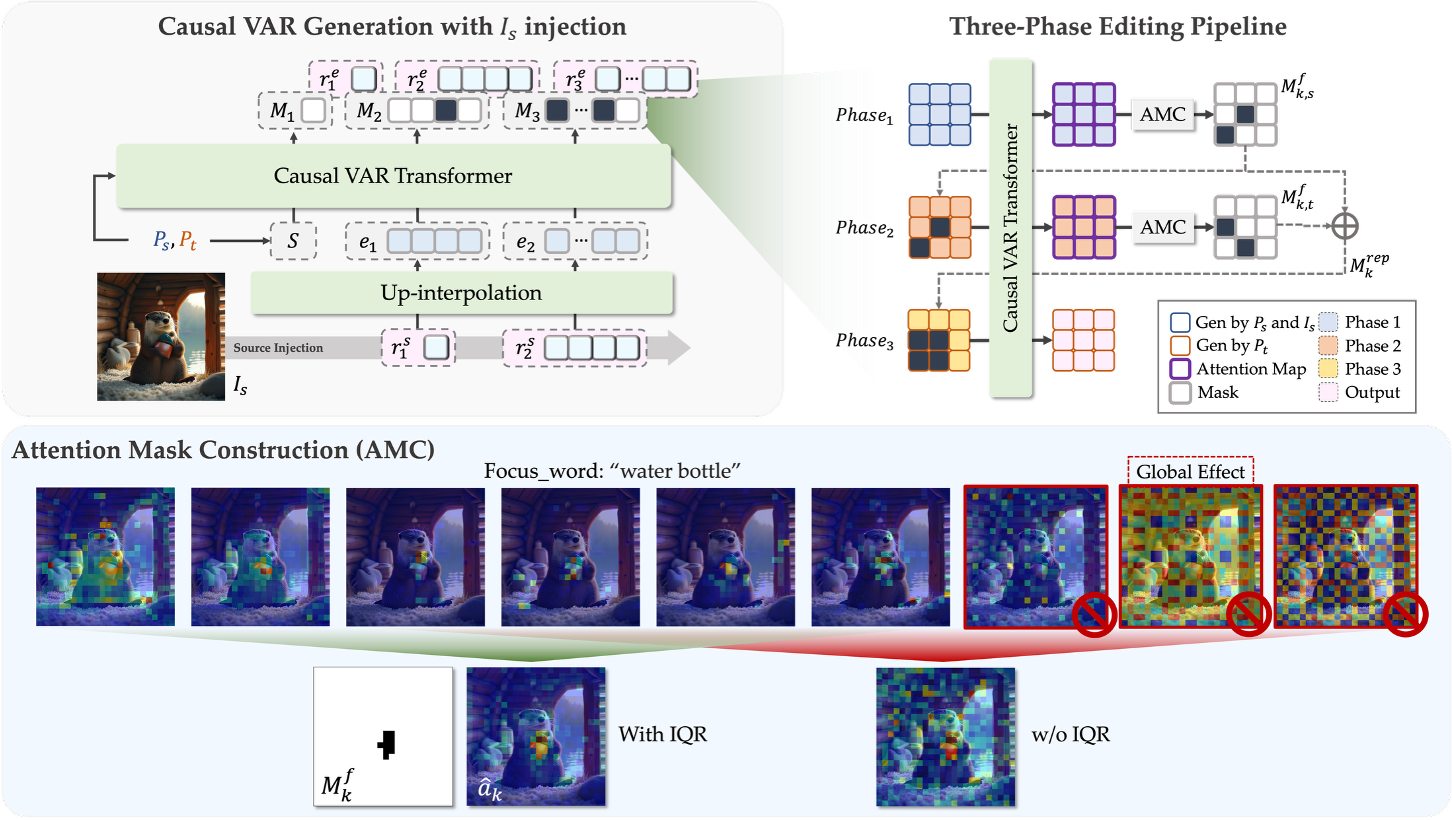
\includegraphics[width=\textwidth]{imgs/pipeline2.png}
    \caption{\textbf{Overview of the proposed editing framework.} \textit{Upper-left:} The source image $I_s$ is encoded into multi-scale discrete tokens $\{r_k^s\}$ via BSQ-VAE; for coarse scales ($k < N$), $r_k^s$ is directly injected into the causal VAR generation to preserve global layout. \textit{Upper-right:} For each scale $k \geq N$, three phases are executed: Phase~1 generates tokens conditioned on $P_s$ to extract $M_{k,s}^{\mathrm{f}}$ and $M_{k,s}^{\mathrm{p}}$; Phase~2 generates tokens conditioned on $P_t$ with background anchoring to extract $M_{k,t}^{\mathrm{f}}$; Phase~3 composes the final output by substituting background positions in $g_k$ with $r_k^s$ according to $M_k^{\mathrm{rep}} = \neg(M_{k,s}^{\mathrm{f}} \cup M_{k,t}^{\mathrm{f}})$. \textit{Bottom:} Detail of Attention Mask Construction (Sec.~\ref{sec:mask_construction}): per-block attention maps $a_{k,b}$ are filtered via IQR to discard positional-bias-dominated transformer blocks, and the retained maps are averaged to produce $\hat{a}_k$, which is then binarized into $M_k^{\mathrm{f}}$ and $M_k^{\mathrm{p}}$.}
    \label{fig:pipeline}
\end{figure*}
